\documentclass[12pt,letterpaper]{article} % For LaTeX2e
\usepackage{amsmath,amsthm,amsfonts,amssymb,amscd}
\usepackage{booktabs}
% \usepackage[nofiglist, notablist]{endfloat}
\usepackage{fullpage}
\usepackage{graphicx}
\usepackage{lastpage}
\usepackage{listings}
\lstset{
	numbers=left,
	numbersep=5pt,
	stepnumber=1,
	tabsize=2,
	showstringspaces=false
}
\usepackage{enumerate}
\usepackage{fancyhdr}
\usepackage{final_project}
\usepackage{hyperref}
\usepackage{mathrsfs}
\usepackage{natbib}
\usepackage{cancel}
\usepackage{times}
\usepackage{tikz}
\usepackage{xcolor}
\usepackage[margin=3cm]{geometry}

% \renewcommand{\efloatseparator}{\mbox{}}




\title{A Social Choice Application}


\author{
Matt Dickenson\\
Department of Political Science\\
Duke University\\
Durham, NC 27708 \\
\texttt{mcd31@duke.edu}
}

\newcommand{\fix}{\marginpar{FIX}}
\newcommand{\new}{\marginpar{NEW}}

\nipsfinalcopy

\begin{document}

\begin{titlepage}

\clearpage
\maketitle
\thispagestyle{empty}

\begin{abstract}
Abstract here.
\end{abstract}
% todo: abstract

\end{titlepage}



\newpage

\section{Introduction}

\subsection{Motivation}

%What is the real-world problem your project will address? 

My proposed project consists of three parts, centered around the implementation of a social choice web application. The Borda count rule serves as a useful voting method for both normative and pragmatic reasons, although it is manipulable. Monte Carlo simulations will be used to estimate the probability of encountering undesirable outcomes and paradoxes using this method. The application can be used for data collection in future research projects, and to enhance public understanding of and familiarity with applied social choice.

Viewing the group decision as an elicitation problem helps to motivate the application.
% todo: explain motivation


\subsection{Problem Definition} 

%Define this problem. What question are you trying to
%solve? What is the goal of the project?

The software application will be useful for a group coordinating on a single outcome by aggregating their preferences, e.g. selecting a movie for a night out with friends. A user creates a movie poll by supplying candidate options (movies) and voters (a list of email addresses to be contacted). A unique link is then sent to each voter, who supplies her ranking of the choices. When all votes have been recorded, an email is sent to all voters with the outcome (and possibly more info, such as anonymized rankings), and a link where they can indicate their satisfaction with the outcome.

One goal for this application is ease of use, in order to set it apart from available online survey applications.\footnote{E.g. \url{http://surveymonkey.com} and \url{http://doodle.com}.} If a user does not submit preferences by a pre-specified deadline, her preferences will be imputed by a default ranking, such as critics' ratings of the candidate movies on \href{http://rottentomatoes.com}{Rotten Tomatoes}. Other desiderata for the voting procedure are discussed in the next section.


\section{A Social Choice Application}



\subsection{Voting Methods}

Desirable properties of the voting method for this application arise from both normative and pragmatic concerns. Anonymity and neutrality ensure that the names of the voters and candidates, respectively, do not influence the outcome. Candidates can be presented to voters in a randomized order to ensure that the format of the list does not bias results. Unanimity requires that if candidate $A$ is preferred over $B$ by all voters, $B$ should not win. The universal domain of potential ballots will be considered in the Monte Carlo simulations, to ensure that the application works with any opinion a voter might entertain about the candidates. Finally, we desire a rule with reinforcement, so that if disjoint sets of voters select the same winner, that candidate should win when the voters are pooled. Practically, this ensures that two small groups of friends who use the app and arrive at the same movie should also have seen that movie if they voted as a single group.
% non-dictatorial? 
% anonymity
% neutrality
% unanimity
% universal domain
% reinforcement

If there are two candidates, the only social decision method that satisfies neutrality, anonymity, and positive responsiveness (if a candidate is tied for the win and moves up in rankings, it will become the winner) is majority rule \citep{may1952}. Less strict conditions, such as Pareto optimality, also motivate the use of majority rule even if positive responsiveness is thought to be too strict \citep{acsan2002,j2003majority}. If there are more than two candidates, only a scoring rule will satisfy anonymity, neutrality, reinforcement, and continuity (if two subgroups of voters select different winners, then there is some number $k$ such that $k$ copies of the first subgroup plus a single copy of the second subgroup will elect the first group's winner) \citep{young1975}. Scoring rules have the additional advantage of being computationally easy.

What voting rule should we choose? Borda count chooses the majority alternative (whenever it exists), and satisfies anonymity, neutrality, unanimity, and reinforcement. A major downside of the Borda rule is that it is easily manipulable \citep{bartholdi1989computational}. However, for a particular type of manipulation (Constructive Coalitional Weighted-Manipulation), manipulating Borda is NP-complete for three candidates, and it is NP-hard for another manipulation (Constructive Individual Unweighted-Manipulation) under uncertainty about others' votes \citep{conitzer2007elections}. More than three candidates should be present for most use cases of the application proposed here. To assess the relative merits of using Borda in this application, Monte Carlo simulations will estimate its vulnerability to manipulation.

% conitzer2003universal
% conitzer2007elections
% xia2009complexity

\subsection{User Experience}

The application described above has been implemented using the Rails framework in the Ruby language. Although the application has not been deployed publicly, the screenshots in Figure \ref{example-screens} give a sense of the user experience. The basic usage process is as follows:
\begin{enumerate}
\item Upon arriving at the homepage, a user is invited to create a poll by supplying candidate options (movie-showtime-location tuples drawn from the Fandango API--see the left pane of Figure \ref{example-screens})
\item The user then invites voters by supplying their names and email addresses
\item An email is sent to each voter inviting her to participate in the poll
\item If the voter chooses to cast a vote, she clicks the unique link in the email (to avoid the need for remembering the password for a user account) and is taken to the voting page (right pane of Figure \ref{example-screens})
\item When all votes are recorded or a deadline has been reached (minimum of one hour before the first canddiate showtime), an email is sent to all voters with the outcome
\end{enumerate}


\begin{figure}[h!]
 \begin{center}
  \begin{minipage}{0.45\textwidth}
    \begin{center}
      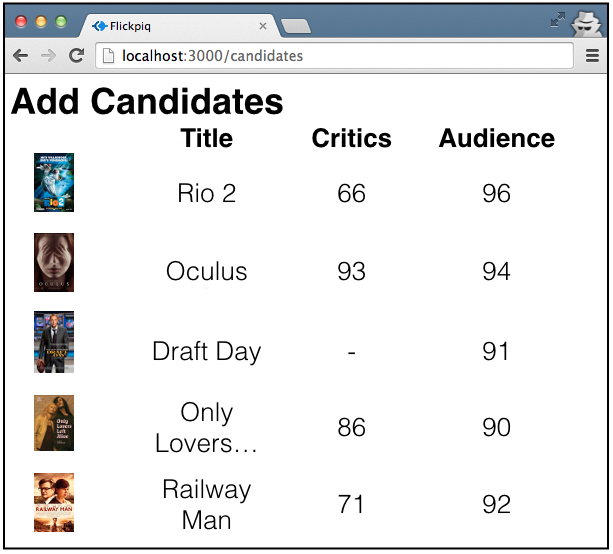
\includegraphics[scale=0.25]{../graphics/add-candidates.png}
    \end{center}
  \end{minipage}
  \hspace{0.05\textwidth}
  \begin{minipage}{0.45\textwidth}
    \begin{center}
      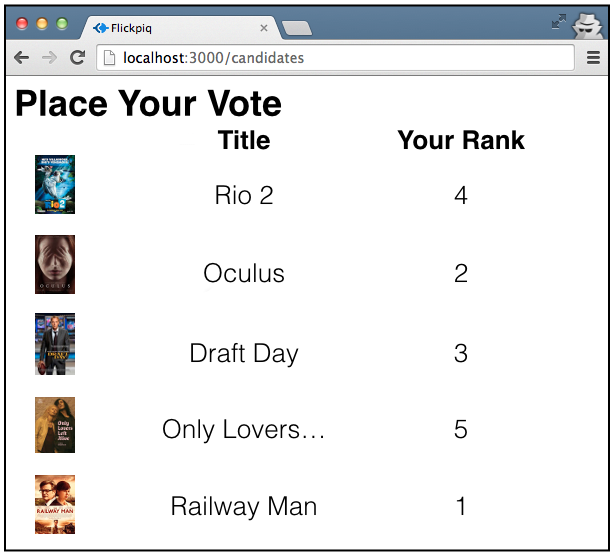
\includegraphics[scale=0.25]{../graphics/place-vote.png}
    \end{center}
  \end{minipage} \\
  \caption{Example screens for poll creator to add candidate movies (left) and for voter to rank candidate movies (right).}
  \label{example-screens}
 \end{center}
\end{figure}



\subsection{Complexity of Elicitation}

How does using this application improve the process of selecting a movie for a group outing? One advantage of this method is that it reduces the average complexity of preference elicitation. When a group coordinates directly over email, there are several disadvantages. First, the pool of voters is not pre-defined: anyone could be added to or omitted from the email conversation at any time. Second, the domain of candidates is not fixed: a new candidate could be added at any time (even when the group is nearing a consensus), extending the time to elicitation exponentially. Third, preferences are expressed in sequence, leading to potential cascading effects resulting in suboptimal outcomes. 
% todo: cite literature on cascading/herd behavior


\section{Simulation and Analysis}

% What will your results show? How will you quantify how well this 
% approach answered the question? What other models/methods will you 
% compare these results against? How will you validate the answers 
% and your uncertainty in the answers?

\subsection{Manipulation Method}

\subsection{Simulation Parameters}

\subsection{Results and Interpretation}

\subsubsection{Frequency of Manipulation}
% > mean(veto$manip)
% [1] 0.8
% > mean(borda$manip)
% [1] 0.187
% > mean(plurality$manip)
% [1] 0.02148
% > mean(veto$manip)
% [1] 0.8

\begin{figure}[h!]
\begin{center}
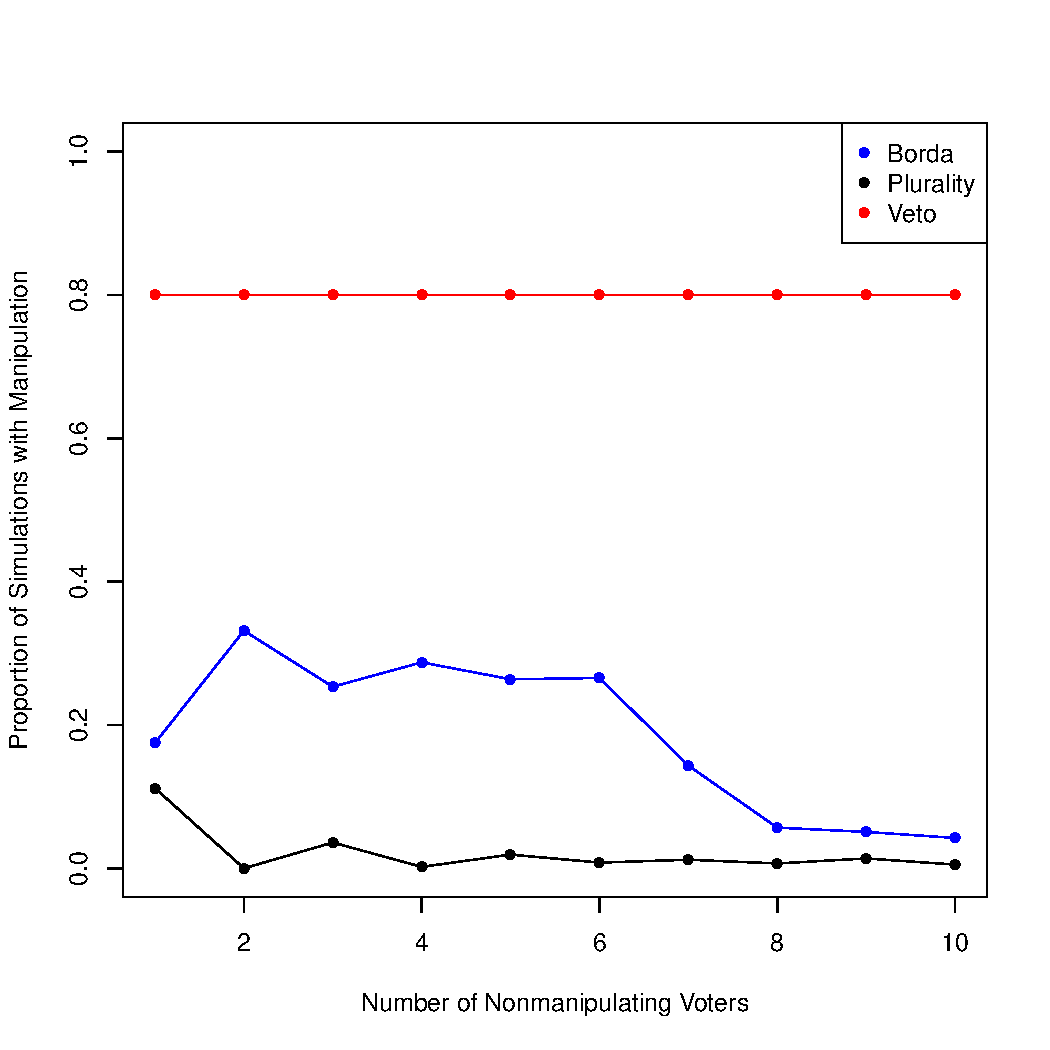
\includegraphics[scale=0.4]{../graphics/manipulation-frequency.pdf}
\caption{Observed frequency of manipulation by voting rule and number of non-manipulating voters.}
\label{manipulation-frequency}
\end{center}
\end{figure}

\subsubsection{Utility With and Without Manipulation}

\begin{center}
\begin{table}
\caption{Average utilities by scenario}
\label{table:utilities}
\begin{tabular}{lcccc}
\multicolumn{1}{c}{} & \multicolumn{2}{c}{Manipulator} & \multicolumn{2}{c}{Nonmanipulator} \\
\multicolumn{1}{c}{} & With Manipulation & Without Manipulaiton & With Manipulation & Without Manipulaiton \\
\hline
Borda     & .58 & .44 & .43 & .76 \\
Plurality & .55 & .44 & .40 & .72 \\
Veto      & .51 & .55 & .60 & .62 % weird, but higher max w/manip
\end{tabular}
\end{table}
\end{center}

\begin{center}
\begin{figure}[h!]
\begin{minipage}{0.45\textwidth}
\begin{center}
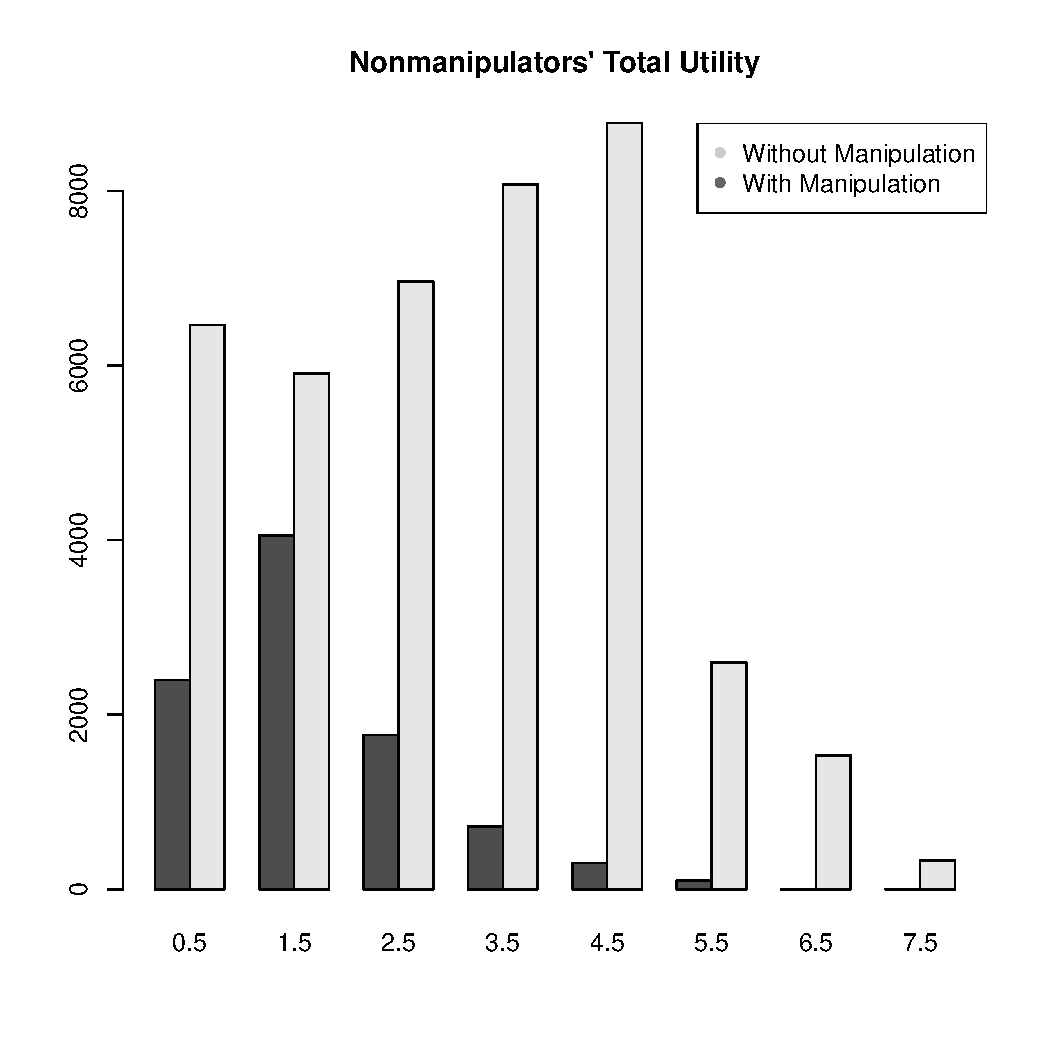
\includegraphics[scale=0.4]{../graphics/nonmanipulators-utilities.pdf}
\end{center}
\end{minipage}
\hspace{0.05\textwidth}
\begin{minipage}{0.45\textwidth}
\begin{center}
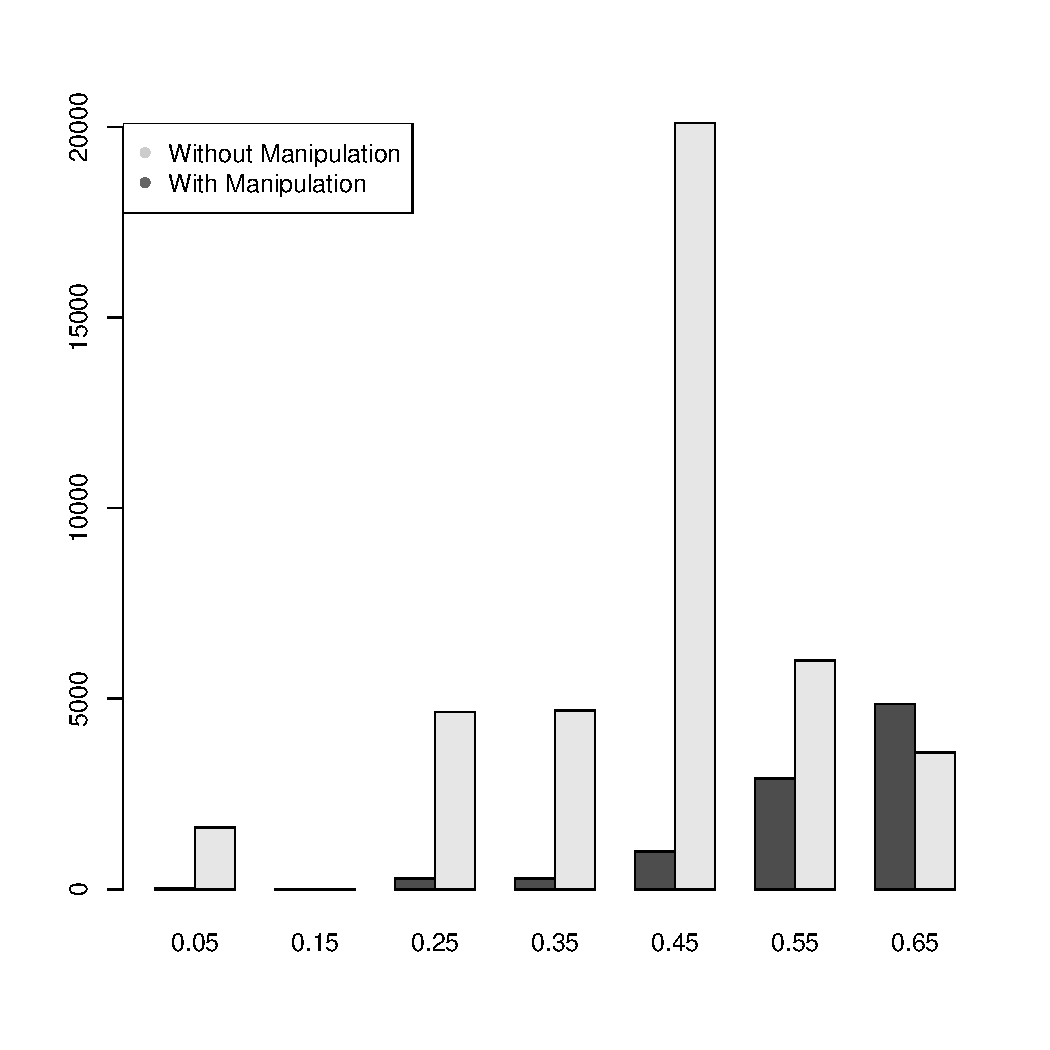
\includegraphics[scale=0.4]{../graphics/manipulator-utilities.pdf}
\end{center}
\end{minipage}
\caption{Nonmanipulators' average utilities (left) and manipulator's utilities (right) with and without manipulation for Borda count simulations.}
\label{nonmanip-manip-utils}
\end{figure}
\end{center}


\section{Related Work}

\section{Conclustion}

Implementing a web application where users can employ Borda voting to coordinate on a group outcome, such as which movie to attend, will help extend the use of social choice to a popular setting. Soliciting satisfaction ratings after the election will help to indicate whether the application is successful and merits wider use. Monte Carlo simulations will estimate the sensitivity to manipulation relative to other rules. 



\subsubsection*{Acknowledgments}

Thanks to Michael D. Ward and National Science Foundation Grant \#3331808 for support during this project. Any conclusions or errors are the sole responsibility of the author.

\newpage
\subsubsection*{References}

% CITE A LOT. Any unreferenced methods, prior work, or biological phenomenon, unless it is textbook-common, will be penalized.


\begingroup
\renewcommand{\section}[2]{}
\bibliographystyle{unsrt}
\bibliography{/Users/mcdickenson/Documents/Templates/RefLib.bib}
\endgroup

\end{document}
